Outra forma de construir soluções boas para o MCSP é utilizando meta-heurísticas, i.e., algoritmos de otimização que utilizam aleatorização em conjunto com busca local \cite[p.~4]{yang_nature-inspired_2010}. Antes de aplicar algum dos vários algoritmos conhecidos, no entanto, é necessário representar as instâncias do problema utilizando uma estrutura de dados eficiente e adequada para tais procedimentos. Encontrar uma boa representação para problemas complexos, como esse, é uma etapa desafiadora, mas que pode simplificar muito a resolução.

Desenvolvemos uma representação baseada em um grafo de substrings comuns \cite{ferdous_solving_2013}, adaptando a representação para arestas múltiplas e ignorando as substrings de tamanho unitário.

\begin{definition}
    Dado um par de strings balanceadas $A$ e $B$ de tamanho $n = \abs{A} = \abs{B}$, temos o \textbf{grafo de substrings comuns} $G_{A,B}(V,E,\varphi)$ de $A$ em $B$ onde:
    
    \begin{enumerate}[
        label = {\alph*)},
        ref = \thedefinition.\alph*,
        parsep = 0pt,
        itemsep = 0.2em,
        topsep = 0pt
    ]
        \item os vértices são dados pelos índices da string $A$: \[
            V = \set{1, \ldots, n} = I_n
        \]

        \item as arestas representam um bloco não-trivial (mais de um caractere) e suas posições como substring de $A$ e $B$: \[
            E = \set{e_{p, q, k} \mid A_p \ldots A_{p + k - 1} = B_q \ldots B_{q + k - 1} ~\text{ e }~ k \geq 2}
        \]

        \item as arestas ligam os caracteres inicial e final de $A$ no bloco: \[
            \varphi\left(e_{p, q, k}\right) = \set{p, p + k - 1}
        \]
    \end{enumerate}
\end{definition}

Note que cada par de bloco representado por uma aresta pode ser utilizado na construção de uma partição comum entre as strings. Arestas paralelas indicam que existe mais de uma substring em $B$ igual à substring de $A$ formada pelos caracteres entre suas extremidades. Um exemplo da representação pode ser visto na \Cref{fig:grafo}.

É importante ressaltar que blocos de apenas 1 caractere não são considerados. Como as strings de entrada são balanceadas e os blocos dos pares são idênticos, ao partir de uma partição comum incompleta, podemos completá-la com todos os caracteres não contidos na partição comum como blocos unitários. Não considerar tais blocos reduz consideravelmente o número de arestas da representação, e consequentemente possibilita algoritmos mais eficientes.

\begin{figure}
    \centering
    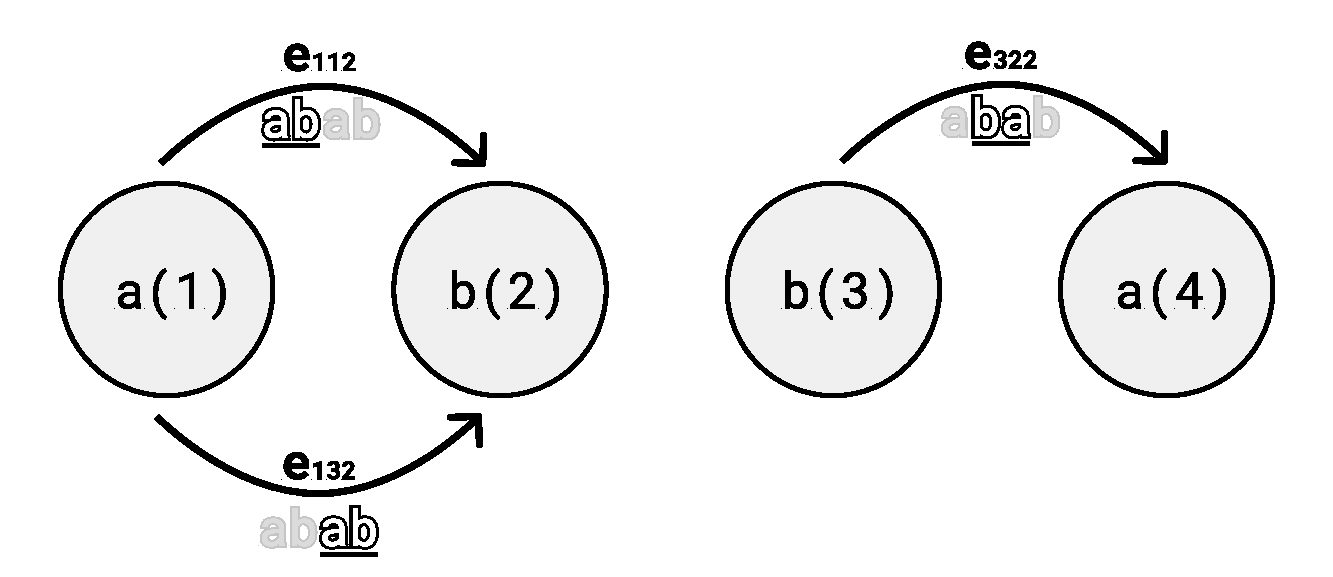
\includegraphics[width=0.8\textwidth]{images/grafo.pdf}
    \caption{Grafo representando a instância (\texttt{"abba"}, \texttt{"abab"}).}
    \label{fig:grafo}
    \todo[inline]{Trocar a figura}
\end{figure}

\subsection{Construindo partições} \label{sec:construindo-particoes}

    A partir de uma sequência ordenada das arestas da representação de uma instância do MCSP, podemos construir partições da seguinte forma: para cada aresta, na ordem dada, incluímos os dois blocos à partição comum se nenhum deles coincide com caracteres contidos em blocos que foram incluídos. Ao fim do processo, cria-se blocos unitários para todos os caracteres não contidos em um bloco. Dessa forma, uma permutação do conjunto de arestas do grafo representa uma única partição comum entre as strings de entrada do problema.

    É válido ressaltar duas propriedades dessa representação. Primeiramente, nem todas as possíveis partições possuem uma permutação correspondente, já que os blocos unitários são omitidos. Tais partições, no entanto, não são as mais interessantes para o MCSP, já que buscamos partições menores.

    Em segundo lugar, note que a partição comum formada por uma permutação das arestas não é única: podemos trocar de posição arestas vizinhas que não são utilizadas, de forma que o mesmo resultado é obtido.

\subsection{Aplicação da representação}

    Com a construção dessa representação, agora o MCSP se reduz a encontrar uma forma de ordenar as arestas de forma que a partição comum resultante seja a menor possível. Isso significa que o reduzimos a um problema de permutação. Algoritmos de otimização que atuam em um espaço de busca contínuo podem ser utilizados para esse tipo de problema aplicando um sistema de pesos que assumem valores reais \cite[p.~661]{marti_handbook_2018}. Relacionamos o vetor de arestas com um vetor de pesos de mesmo tamanho, de forma que a ordenação das arestas pelos valores dos pesos correspondentes forma a permutação correspondente àqueles valores. Como cada peso é uma componente no espaço de busca, podemos nos referir ao vetor de pesos também como posição (e à sua variação, como velocidade).
